% ------------------------------------------------------------------
\section{The Born-Oppenheimer Approximation}
\label{sec:born-oppenheimer}
In order to simplify --- and in many cases, make possible --- quantum calculations of large atomic systems, the difference in weight of the electrons and the nuclei\footnote{\mytilde 4 orders of magnitude for hydrogen and more for the heavier elements.} is exploited by performing the calculations in two steps.
First, while the nuclei are kept motionless by excluding their kinetic operator from the Hamiltonian (\fref{eq:hamiltonian}), the electronic wavefunction and energy are determined followed by a calculation for the motion of the nuclei.
The assumption is, essentially, that for any motion of the nuclei, the electrons will move instantly and relax to their ground state to accommodate.
This is commonly known as the Born-Oppenheimer approximation.~\cite{born-oppenheimer-1927}

\begin{figure}[h]
  \begin{center}
    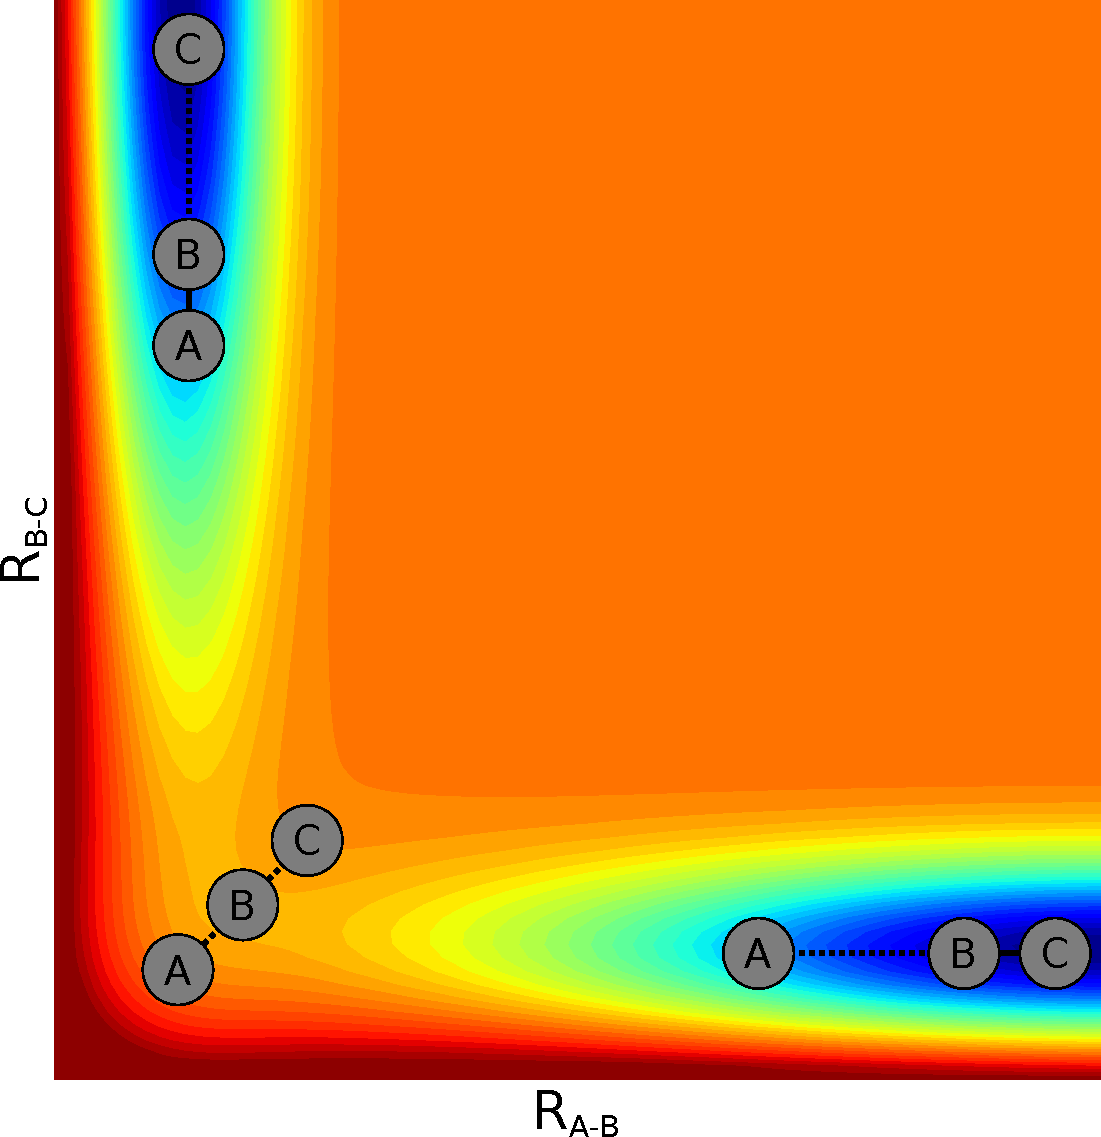
\includegraphics[width=0.6\linewidth]{three-atom-pes}
\parbox{0.85\linewidth}{
    \caption{
A schematic example potential energy surface.
The axes are functions of nuclear positions, showing the distance between atoms A and B on the one hand and B and C on the other.
\expand
}
\label{fig:dimer-force-overview}
}
  \end{center}
\end{figure}


This decoupling allows for a mapping of the potential energy as a function of the nuclear coordinates (commonly referred to as the potential energy surface or PES), as opposed to the continuum of PESes which exist should the motion of the nuclei and electrons be determined simultaneously.
PESes are, generally, not known \textit{a priori} and much effort is spent on traversing them to discover interesting features, such as minima, which represent stable atomic structures, or, as we shall see below, reaction pathways.

%\url{http://www.search.com/reference/Born-Oppenheimer_approximation}
%Should be bad for metallic systems but has proved useful nevertheless. \footnote{see \url{http://www.nature.com/nmat/journal/v6/n3/pdf/nmat1846.pdf}}
%\url{http://www.jhu.edu/~chem/yarkony/research.html} specializes in non-BOA calculations.

All the work carried out in this thesis employs this approximation.
